\section{Analisis dan Evaluasi}
\label{sec:Analisis & Evaluasi}
\setlength{\parskip}{0pt}
% Prevent footnote splitting dan flexible page layout
\interfootnotelinepenalty=10000
\clubpenalty=10000
\widowpenalty=10000
\raggedbottom

Setelah memetakan substansi kedua artikel Budiawan secara rinci, tibalah saatnya menimbang secara kritis kekuatan dan kelemahan argumentasinya. Analisis ini ditempatkan dalam kerangka literatur \textit{fiscal capacity} yang lebih luas—terutama dengan mempertimbangkan paradoks sumber daya fiskal yang telah kita singgung di pendahuluan. Paradoks ini, sebagaimana yang akan kita lihat, bukan sekadar soal teknis; ia adalah simpul persoalan yang—anehnya—terus kembali dalam wacana fiskal Indonesia, seolah menjadi motif berulang dalam narasi kebijakan pajak kita.

\subsection{Kekuatan Artikel: Data yang Meyakinkan dan \textit{Political Timing} yang Tepat}

Kekuatan utama pendekatan Budiawan terletak pada ketajamannya membaca lanskap empiris dan celah retorika kebijakan. Survei \textit{Kompas} yang dikutipnya bukan hanya metodologis—625 responden, 38 provinsi, \textit{margin of error} ±3,92 persen—tetapi juga politis dalam efeknya. Hasil survei yang menunjukkan penolakan publik secara \textit{cross-cutting} memberi legitimasi pada klaim bahwa resistensi terhadap kenaikan tarif bukanlah ekspresi emosional yang temporer, melainkan refleksi dari kegelisahan yang lebih dalam dan sistemik.

Budiawan juga jeli memanfaatkan perbandingan internasional. Kondisi yang Ia tampilkan: Thailand dengan GST 7 persen memiliki tax ratio 15,14 persen, sementara Indonesia dengan PPN 11 persen hanya 10,4 persen. Di sini, Budiawan berhasil melakukan \textit{reframing}: alih-alih bertanya “perlukah tarif dinaikkan?”, ia menggeser fokus menjadi “mengapa sistem kita gagal memobilisasi penerimaan?”—suatu pergeseran yang subtil tetapi strategis.

\textit{Strategic positioning} kedua artikel juga menunjukkan kejelian politik yang patut dicatat. Artikel pertama hadir sebagai suara akademis yang kredibel di tengah riuhnya opini publik, sementara artikel kedua memberikan validasi empiris atas keputusan pemerintah tanpa terkesan oportunistik. \textit{(Timing}-nya terasa tepat: Budiawan berhasil menempatkan dirinya sebagai peneliti yang konsisten dengan analisis berbasis bukti di tengah polarisasi—posisi yang tidak mudah dipertahankan di lanskap kebijakan Indonesia.)

\subsection{Paradoks Fundamental: Masalah "Ayam dan Telur" yang Tak Kunjung Terurai}

Artikel tersebut tajam, tetapi dibaliknya, tersembunyi paradoks yang tak kunjung terurai (yang sudah disinggung pada bagian \hyperref[sec:Pendahuluan]{\textit{Pendahuluan}}). Budiawan menyarankan bahwa penguatan institusi adalah prasyarat untuk peningkatan kapasitas pajak. Akan tetapi, reformasi institusi itu sendiri memerlukan sumber daya—yang ironisnya, baru bisa diperoleh bila penerimaan fiskal (dalam hal ini pajak) telah membaik

Kedua artikel Budiawan, dengan cara yang hampir tidak disengaja, menghadirkan \textit{puzzle} yang akrab bagi siapa pun yang pernah bergulat dalam perdebatan fiskal Indonesia: bagaimana mungkin kita membenahi sistem perpajakan—yang, implikasinya, juga berarti memperkuat institusi negara dan membangun kapasitas negara (\textit{state capacity})—tanpa terlebih dahulu memiliki sumber daya untuk membiayai perbaikan itu sendiri? Sumber daya itu pada gilirannya diharapkan datang dari penguatan \textit{tax capacity}—yang, sebagaimana diingatkan Brautigam et al. (2008), adalah sumber penerimaan paling andal dan berkelanjutan bagi \textit{statebuilding}.  
\catatan{Paradoks ini mengingatkan pada apa yang oleh literatur ekonomi politik disebut \textit{bootstrapping problem}—membangun institusi pajak butuh dana, tetapi dana itu hanya tersedia jika institusi pajak sudah kuat. Sebuah sirkularitas yang membuat kebijakan terjebak dalam pusaran mandek: untuk menggerakkan A, perlu B; tapi B hanya tersedia jika A sudah berjalan.}  

Studi IMF (2023), yang hasilnya dipaparkan pada \hyperref[tab:tab:tax_potential_effort]{\textit{Bagan}~\ref{tab:tax_potential_effort}}, menunjukkan bahwa negara-negara LIDCs memiliki potensi pajak sekitar 19,9 persen PDB, tapi realisasinya hanya 12,1 persen. Indonesia bahkan lebih rendah dari itu. Maka persoalannya bukan hanya soal moral atau komitmen birokratik—tapi soal struktur: sistem kita tidak diberi cukup "amunisi" untuk bertempur. Reformasi kelembagaan, betapapun esensialnya, tidak datang tanpa ongkos. Modernisasi sistem informasi perpajakan menuntut investasi bernilai miliaran rupiah; perbaikan birokrasi—termasuk penyediaan insentif agar aparatur tak tergoda rente—memerlukan skema kompensasi yang kompetitif; dan investasi jangka panjang dalam sumber daya manusia hanya mungkin berlangsung dengan dukungan anggaran yang berkelanjutan \citep{chang_2011_institutions}.\catatan{Ironisnya, semua itu membutuhkan kapasitas fiskal yang justru belum kokoh—lingkaran yang sulit diputus.}  

\begin{table}[hbt!]
\caption{Potensi Pajak dan \textit{Tax Effort} Berdasarkan Kelompok Negara (2020)}
\label{tab:tax_potential_effort}
\centering
\begin{tabular}{1111}
\resizebox{\columnwidth}{!}{%
\begin{tabular}{@{}lll@{}}
\toprule
\multicolumn{1}{c}{\textbf{Kelompok Negara}} & \multicolumn{1}{c}{\textbf{Potensi Pajak (\%PDB)}} & \multicolumn{1}{c}{\textbf{Peneriman Aktual (\% PDB)}} \\ \midrule
Advanced Economies (AEs)                & 26,0 & 24,6 \\
Emerging Market Economies (EMEs)        & 22,5 & 16,6 \\
Low-Income Developing Countries (LIDCs) & 19,9 & 12,1 \\ \bottomrule
\end{tabular}%
}
\end{tabular}
\floatnote{\textit{Sumber:} IMF (2023). \textit{Tax effort} didefinisikan sebagai rasio antara penerimaan aktual dan potensi pajak. Nilai yang semakin mendekati 1,0 menunjukkan efektivitas mobilisasi pajak yang semakin tinggi.}
\end{table}   

\subsection{Konservatisme Fiskal yang Tidak Disadari}
Di tengah kenyataan bahwa \textit{tax-to-GDP ratio} Indonesia masih stagnan, bahkan di beberapa periode pascapandemi cenderung menurun, muncul pertanyaan yang sulit dielakkan: dari mana sumber daya fiskal untuk membiayai reformasi tersebut berasal? Pilihan yang secara administratif paling mudah—dan yang juga menjadi pangkal kegelisahan publik—adalah mendorong kenaikan penerimaan pajak melalui tarif umum PPN.

Evaluasi yang adil juga harus mengidentifikasi potensi bias dalam pendekatan Budiawan. Dengan menekankan optimalisasi sistem yang ada dan menghindari diskusi tentang \textit{substantive tax increases}, ia mungkin secara tidak sadar mengafirmasi \textit{status quo} dan menghindari reformasi fiskal yang lebih \textit{bold} tapi diperlukan.

Dalam konteks kebutuhan investasi besar—baik untuk infrastruktur, penanggulangan perubahan iklim, maupun pengembangan sumber daya manusia—pertanyaan mengenai kecukupan (\textit{adequacy}) dari ruang fiskal yang ada menjadi penting. Literatur menunjukkan bahwa banyak negara berkembang perlu memperluas \textit{fiscal space} secara signifikan untuk mencapai target pembangunan \citep{murshed_2020_fiscal}.

Pendekatan yang terlalu fokus pada \textit{efisiensi} dari sistem yang ada, tanpa mengalamatkan \textit{kecukupan} dari \textit{tingkat penerimaan yang dibutuhkan secara menyeluruh},  berpotensi tidak memadai untuk menjawab kebutuhan pembangunan Indonesia. \catatan{Ini adalah observasi, yang tidak unik, tentang mengenai konsekuensi tak terduga dari kerangka analisis yang sering orang pilih}. Kadang-kadang, apa yang tampak sebagai pragmatisme \textit{incremental} justru dapat membatasi \textit{policy imagination} tentang apa yang mungkin dan perlu dilakukan. Di sinilah terlihat kehati-hatian Budiawan—atau, jika menggunakan istilah lain, konservatisme fiskal. Alih-alih mengadvokasi terobosan yang bersifat ekspansif, ia lebih memilih menekankan optimalisasi tata kelola. Penting, tentu saja, tetapi pertanyaannya: apakah itu cukup? Atau, meminjam peribahasa lama, bisakah kita mengubah wajah kebijakan hanya dengan merapikan cermin, tanpa menyentuh ruang di baliknya?

Sebelum menilai lebih jauh, perlu diakui bahwa langkah kenaikan tarif umum PPN yang sempat menuai resistensi publik sesungguhnya merupakan kebijakan yang, dari sisi penerimaan, cukup rasional. \textit{Tax-to-GDP ratio} Indonesia yang stagnan selama lebih dari satu dekade, dengan kebutuhan pembiayaan pembangunan yang kian mendesak, menuntut adanya sumber pendapatan yang relatif cepat, stabil, dan secara administratif dapat diandalkan. Kenaikan PPN tahun lalu—meski tidak populer—secara teknis adalah langkah yang sulit dihindari. Kontribusi PPN terhadap penerimaan negara cukup signifikan dan relatif tahan terhadap fluktuasi ekonomi \citep{saptono_2022_institutional,arvin_2021_are}. 

Pilihan menaikkan tarif umum PPN sering dianggap langkah yang paling mudah secara administratif—sebagaimana dicatat dalam literatur fiskal \citep{brautigam_2008_taxation, timmons_2005_the, akanbi_2019_state, addison_2018_fiscal, gaspar_2016_tax, iswahyudi_2021_getting}. Alasannya tidak hanya terletak pada kesederhanaan mekanisme: PPN memiliki basis pemungutan yang luas, tingkat kepatuhan yang relatif lebih baik dibanding pajak langsung, dan—ini penting dalam konteks Indonesia—lebih tahan terhadap tantangan informalitas. Dengan lebih dari separuh tenaga kerja masih berada di sektor informal (ILO, 2023) dan estimasi \textit{shadow economy} yang berkisar 19–30 persen PDB (IMF; ADB), basis pajak langsung menjadi sempit dan sulit diawasi. PPN, sebaliknya, dipungut di titik konsumsi formal yang relatif lebih mudah dilacak. Ibaratnya, ini jalur tol fiskal: tanpa perlu menembus hutan belantara informalitas, penerimaan negara tetap mengalir.  

Korelasi antara tingkat pajak dan kualitas institusi—sebagaimana terlihat pada \textit{Gambar}~\ref{fig:pajak_institusi}—terlihat konsisten. Namun, tentu penulis menyadari bahwa korelasi tidak otomatis berarti kausalitas. Peningkatan rasio pajak terhadap PDB, jika hanya dibaca dari grafik, belum tentu menjadi penyebab langsung menguatnya kapasitas institusi. \catatan{Dan di sini, godaan untuk tergesa-gesa menyimpulkan hubungan sebab-akibat memang selalu mengintai.}  

\begin{figure}[hbt!]
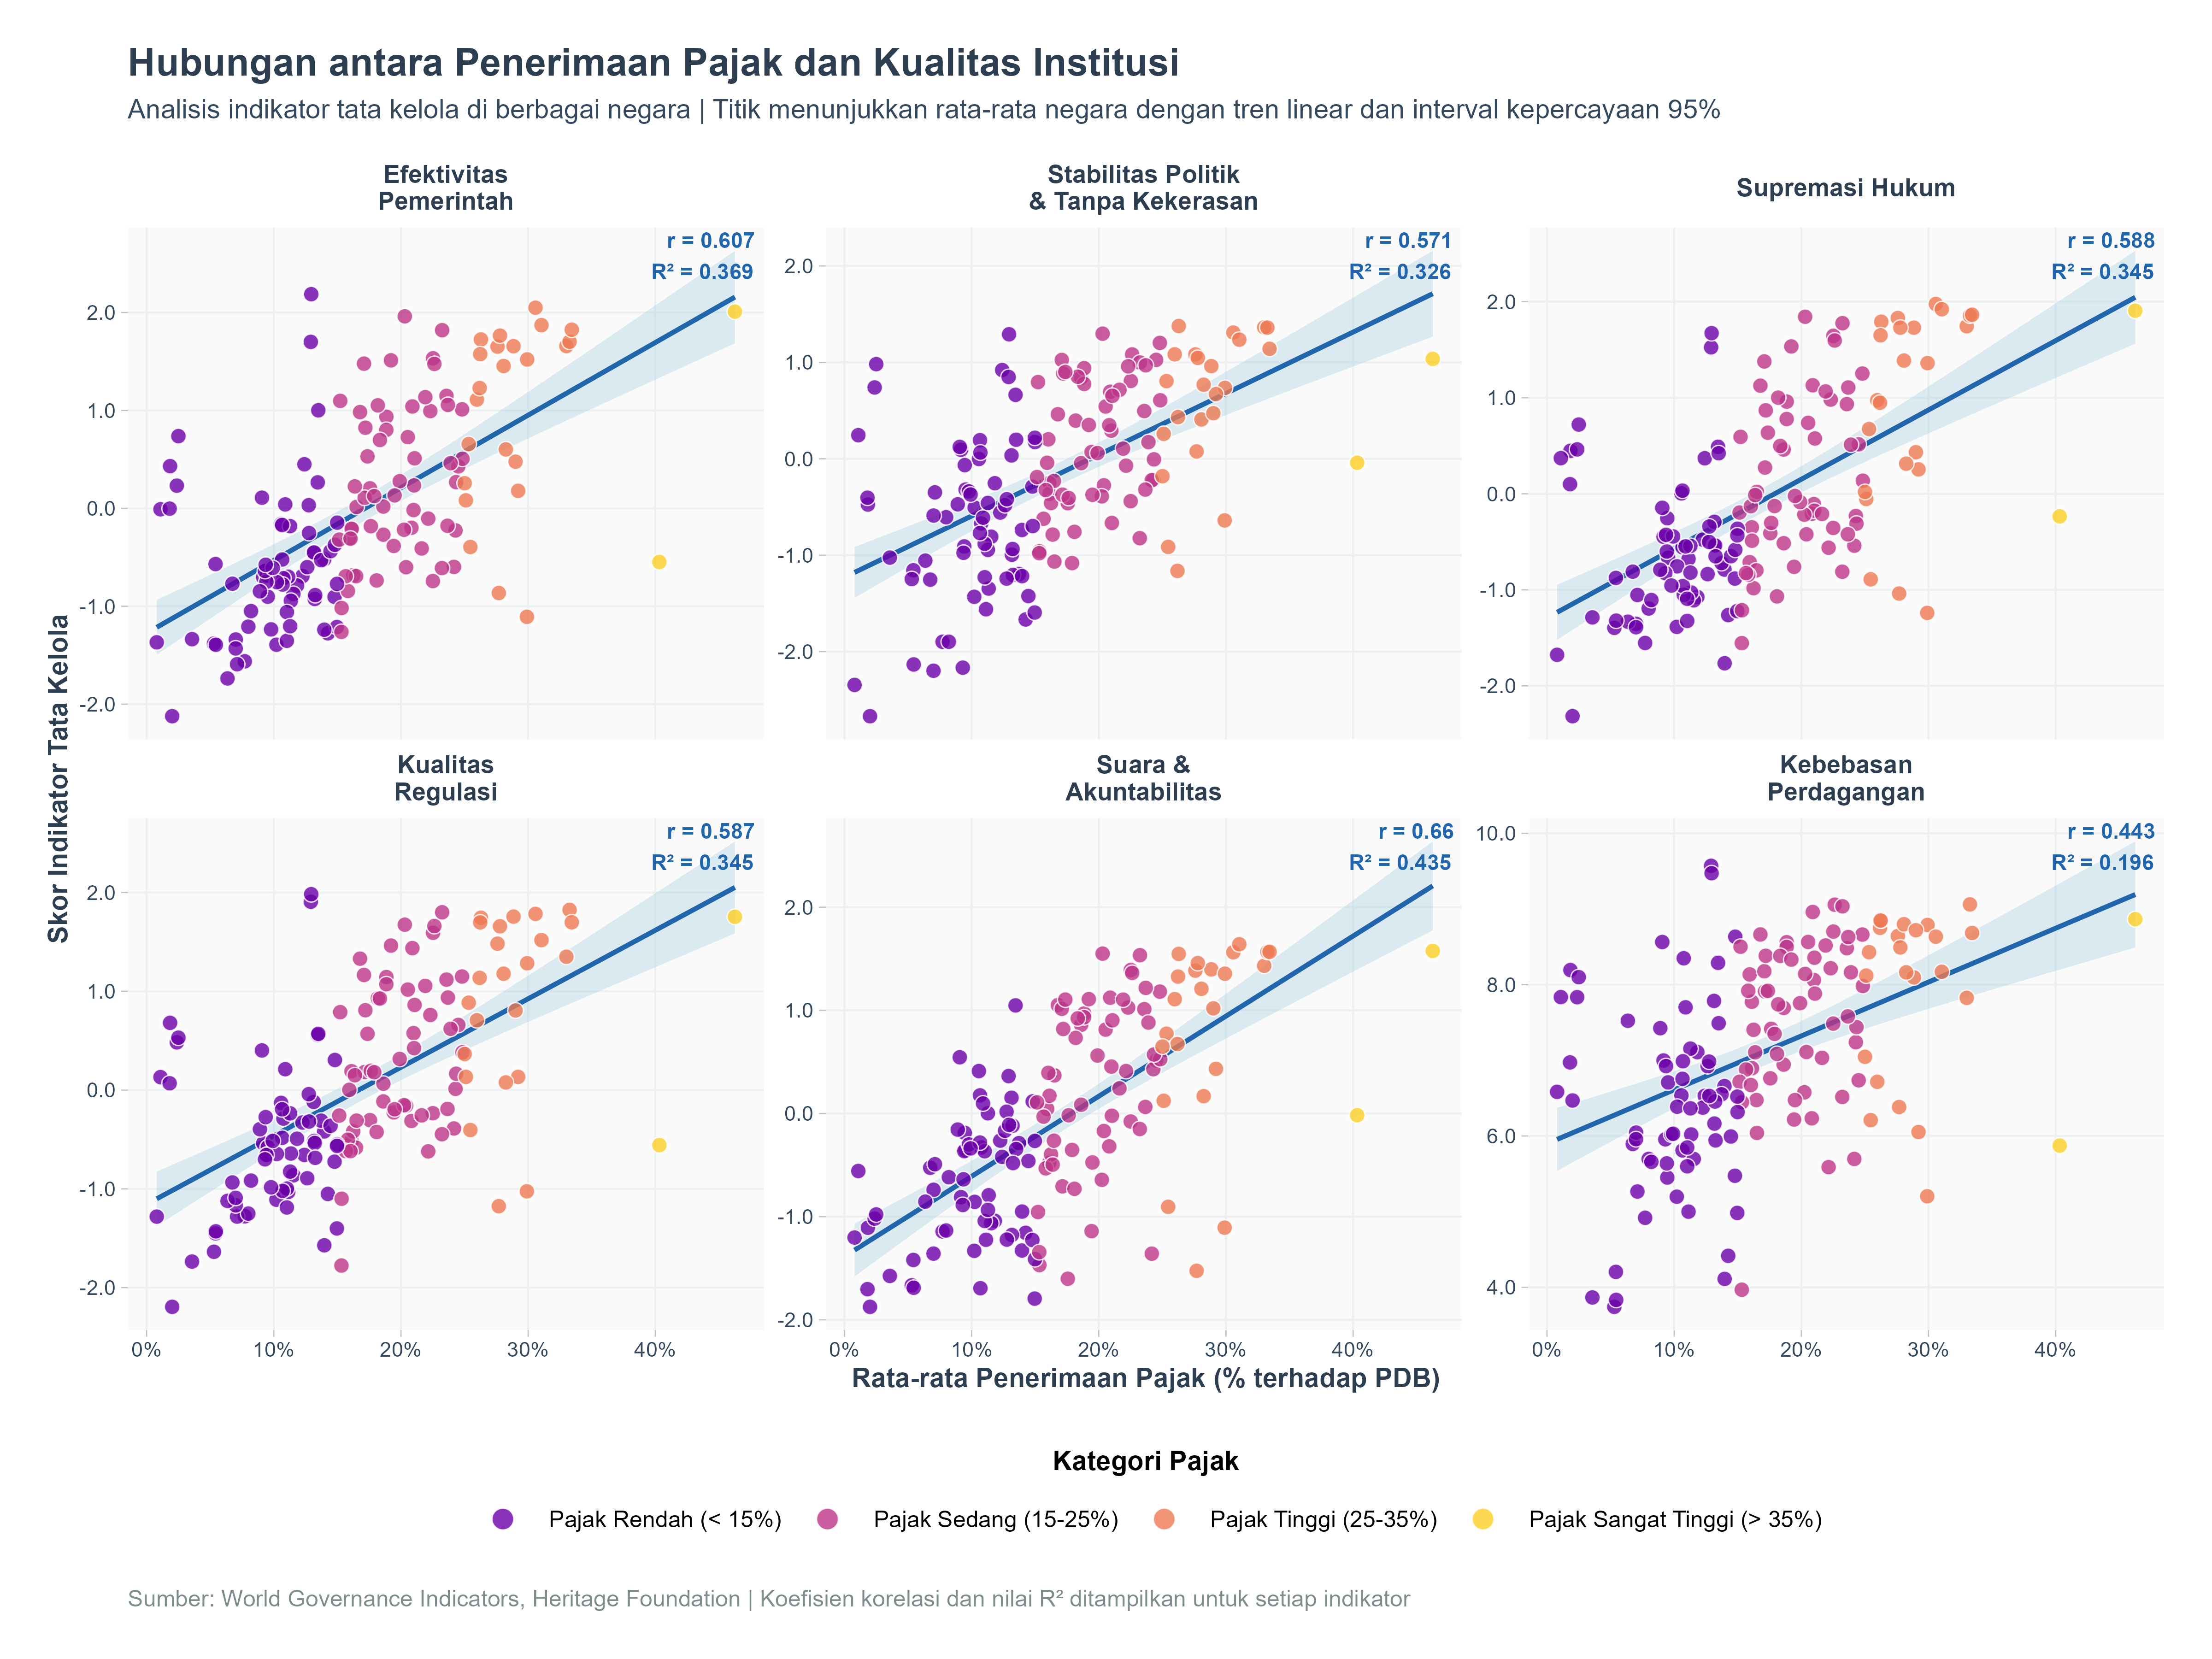
\includegraphics[width=\linewidth]{analisis_pajak_tata_kelola.png}
\caption{Hubungan Antara Tingkat Pajak dan Kualitas Institusi.}
\label{fig:pajak_institusi}

\floatnote{Visualisasi ini menunjukkan hubungan antara persentase penerimaan pajak terhadap PDB dan berbagai indikator tata kelola pemerintahan di negara-negara terpilih. Setiap panel menampilkan regresi linier dan rentang kepercayaan 95\%.
\newline
\textit{Sumber data:} ICTD/UNU-WIDER Government Revenue Dataset (2023); World Governance Indicators (2023); Heritage Foundation (2023). Visualisasi dibuat oleh Penulis menggunakan R.}
\end{figure}

Literatur memberi penjelasan yang lebih hati-hati. \citet{akanbi_2019_state}, melalui panel Granger causality test, menemukan hubungan kausalitas dua arah antara kapasitas pajak dan kualitas institusi. Menggunakan Panel Vector Error Correction Model, ia menunjukkan bahwa keduanya saling memperkuat di berbagai kelompok negara. Artinya, membangun kapasitas pajak dan institusi sebaiknya dilakukan beriringan—bukan menunggu yang satu selesai baru yang lain dimulai.  Arvin et al. (2021) sampai pada kesimpulan serupa, yaitu pertumbuhan ekonomi per kapita di negara-negara berpendapatan rendah dan menengah ke bawah dipengaruhi signifikan oleh penerimaan pajak, belanja pemerintah, dan kualitas institusi—terlepas dari jenis pajak yang digunakan.  Gaspar et al. (2016) menambahkan dimensi menarik: adanya ambang batas (\textit{tipping point}) rasio pajak terhadap PDB (bisa merujuk ke \textit{\hyperref[fig:view]{Gambar 2}}). Mereka menemukan bahwa ketika rasio tersebut mencapai sekitar 12,75 persen, PDB riil per kapita cenderung meningkat tajam dan berkelanjutan dalam dekade berikutnya. Rata-rata negara yang naik dari 12,5 persen menjadi 13 persen \textit{tax-to-GDP} berpeluang memiliki PDB per kapita sekitar 7,5 persen lebih besar dibanding negara sejenis yang tetap berada di bawah ambang tersebut. \textit{Seolah ada “pintu rahasia” yang baru terbuka begitu ambang ini terlampaui.}

Dari sini, ada satu implikasi yang tampaknya luput diperhitungkan Budiawan: konsep \textit{tax tipping point} ini mengindikasikan bahwa negara-negara dengan kapasitas pajak di bawah 12,75 persen dari PDB rawan terjebak dalam \textit{low tax capacity trap} \citep{akanbi_2019_state}. Di bawah ambang ini, kapasitas pajak yang rendah dan institusi yang lemah cenderung berjalan beriringan. Dan keluar dari jebakan ini, sebagaimana disarankan literatur, memerlukan langkah simultan—peningkatan penerimaan dan reformasi kelembagaan—bukan pendekatan sekuensial seperti yang cenderung diimplikasikan Budiawan. Indonesia, dengan \textit{tax ratio} 10,4 persen, berada tepat di zona risiko tersebut. Penelitian IMF menunjukkan bahwa peningkatan efektivitas pemerintahan sebesar satu standar deviasi dapat mendorong potensi pajak sebesar 2,8 poin persentase PDB (dari 19,9 persen menjadi 22,7 persen untuk LIDCs). Pertanyaannya, tentu saja: bagaimana melakukan perbaikan efektivitas pemerintahan itu jika sumber daya fiskalnya sendiri masih terbatas?

\begin{figure}[hbt!]
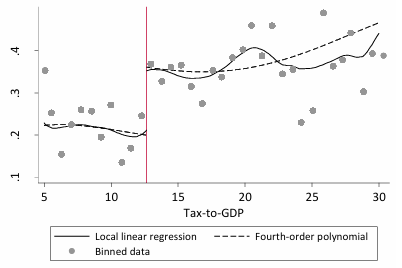
\includegraphics[scale=1.8]{Tax Tipping Point.png}
\caption{Dampak Ambang Pajak terhadap Pertumbuhan PDB Kumulatif 10 Tahun.}
\label{fig:view}
\floatnote{Diagram ini diadaptasi dari \citet{gaspar_2016_tax}, yang menunjukkan hubungan antara rasio pajak terhadap PDB (\textit{tax-to-GDP ratio}) dan pertumbuhan PDB riil kumulatif selama sepuluh tahun pada basis data historis. Titik-titik menggambarkan rata-rata pertumbuhan PDB dalam interval 0,75 poin persentase. Garis penuh merupakan hasil \textit{local linear regression} di kedua sisi ambang 12,65 persen menggunakan \textit{Epanechnikov kernel} dengan \textit{bandwidth} 1,5, sementara garis putus-putus adalah \textit{fourth-order polynomial} dengan pergeseran intersep di titik ambang yang diestimasi.}
\end{figure}

\begin{figure}[hbt!]
\centering
\begin{tikzpicture}[node distance=3cm, thick,  xscale=1.0, yscale=1.2, transform shape]

% Define styles
\tikzstyle{state} = [rectangle, draw, fill=blue!20, text width=3.5cm, text centered, rounded corners, minimum height=1.5em, font=\small]
\tikzstyle{outcome} = [rectangle, draw, fill=green!20, text width=3.5cm, text centered, rounded corners, minimum height=1.5em, font=\small]
\tikzstyle{factor} = [ellipse, draw, fill=yellow!20, text width=2.8cm, text centered, minimum height=1.5em, font=\small]
\tikzstyle{unobs} = [ellipse, draw, fill=gray!20, text width=2cm, text centered, minimum height=1.5em, dashed, font=\small]
\tikzstyle{arrow} = [->, >=latex, thick]
\tikzstyle{doublearrow} = [<->, >=latex, thick]
\tikzstyle{dashedarrow} = [->, >=latex, thick, dashed]

% Layout nodes in a cleaner arrangement
% Top row
\node[factor] (reform) at (-6,6) {Biaya Reformasi};
\node[state] (ins) at (0,6) {Kualitas Institusi};
\node[factor] (trust) at (6,6) {Kepercayaan Publik};

% Middle row
\node[state] (gex) at (-7,3) {Belanja Pemerintah};
\node[unobs] (unobs) at (-3,4) {$U$};
\node[outcome] (peg) at (6,3) {Pertumbuhan Ekonomi};

% Bottom row
\node[factor] (shadow) at (-6,0) {\textit{Shadow Economy}};
\node[state] (tax) at (0,0) {Kapasitas Pajak};
\node[outcome] (revenue) at (6,0) {Penerimaan Negara};

% Main causal relationships dengan path yang lebih jelas
% Bidirectional INS <-> PEG untuk LMICs
\draw[doublearrow] (ins) to[bend right=25] node[midway, right, font=\scriptsize] {LMICs} (peg);

% Direct effects
\draw[arrow] (ins) -- (tax) node[midway, left, font=\scriptsize] {+};
\draw[arrow] (ins) -- (trust) node[midway, above, font=\scriptsize] {+};
\draw[arrow] (trust) -- (tax) node[midway, right, font=\scriptsize] {+};
\draw[arrow] (gex) -- (peg) node[midway, below, font=\scriptsize] {+};
\draw[arrow] (tax) -- (peg) node[midway, below, font=\scriptsize] {+};
\draw[arrow] (tax) -- (revenue) node[midway, below, font=\scriptsize] {+};
\draw[arrow] (shadow) -- (tax) node[midway, below, font=\scriptsize] {-};

% Reform effects
\draw[arrow] (reform) -- (ins) node[midway, above, font=\scriptsize] {+/-};

% Long-run relationship
\draw[arrow, line width=2pt, color=blue!60] (revenue) to[bend right=30] node[midway, below, font=\scriptsize] {Jangka Panjang} (peg);

% Feedback loop
\draw[dashedarrow, color=red!60] (revenue) to[bend left=40] node[midway, left, font=\scriptsize] {feedback} (reform);

% Unobserved confounders dengan path yang jelas
\draw[dashedarrow] (unobs) -- (ins);
\draw[dashedarrow] (unobs) -- (gex);
\draw[dashedarrow] (unobs) to[bend right=15] (tax);

\end{tikzpicture}
\caption{Diagram Kausal: Hubungan Institusi, Kapasitas Pajak, dan Faktor-Faktor Terkait}
\label{fig:integrated_causal}
\floatnote{Diagram ini mengintegrasikan temuan empiris Arvin et al. (2021) dengan faktor-faktor kontekstual tambahan. Variabel disusun dalam tiga tingkat: faktor institusional (atas), proses ekonomi (tengah), dan hasil fiskal (bawah). Garis putus-putus menunjukkan pengaruh variabel tak terobservasi ($U$) dan hubungan feedback.}
\end{figure}

Temuan-temuan ini memperkuat argumen bahwa penguatan tingkat, dalam arti kapasitas pemungutan, pajak bukan sekadar solusi teknis jangka pendek, melainkan bagian dari strategi yang lebih besar—yang pada gilirannya memengaruhi kualitas tata kelola dan kinerja ekonomi secara keseluruhan.

Sebagai penutup bagian ini, penting mengingat perspektif historis yang ditawarkan Brautigam et al. (2008) dalam karya seminalnya tentang \textit{state-building} dan perpajakan di negara berkembang. Ia menegaskan bahwa sistem perpajakan modern di Eropa tidak muncul begitu saja. Ia lahir dari proses negosiasi panjang antara penguasa dan elite ekonomi—di mana pajak ditukar dengan representasi politik dan perlindungan hak properti. 

\begin{quote}
“Taxation is a core governance function. It has the potential to shape relations between state and society in significant and distinctive ways. Tax revenues allow states to provide security and public goods. ‘The history of state revenue production,’ Margaret Levi once wrote, ‘is the history of the evolution of the state.’ For these reasons, taxation should be accorded a central role in analyses of state building.” \citep{brautigam_2008_taxation}
\end{quote}

Indonesia, dengan segala kompleksitas politik dan ekonominya, belum benar-benar melalui proses negosiasi semacam ini hingga tuntas. Mungkin di sinilah letak tantangan kita: bukan hanya soal tarif atau administrasi, tetapi juga tentang membangun kontrak sosial yang membuat pajak dipandang bukan sebagai beban, melainkan sebagai bagian dari kesepakatan bersama dalam membentuk negara yang lebih kuat.

\subsection{Masalah \textit{Transferability}: Vietnam dan Singapura sebagai \textit{False Analogy}?}
Perbandingan dengan Vietnam dan Singapura yang kerap dirujuk Budiawan layak dikaji kembali secara lebih kritis. Vietnam menjalani transisi ekonomi dalam kerangka \textit{political settlement} yang sangat berbeda, dengan dukungan modal asing masif serta konsensus politik yang relatif solid. Reformasi fiskalnya beriringan dengan kebijakan \textit{doi moi} (renovasi ekonomi) yang ditopang bantuan internasional substansial.
\textit{(Konteks ini sulit direplikasi: bukan hanya soal teknis kebijakan, tetapi juga momentum politik yang langka.)}

Singapura, di sisi lain, adalah sebuah \textit{city-state} dengan karakteristik yang hampir tak bisa dibandingkan langsung: perekonomian yang sangat terbuka dan terintegrasi dalam \textit{global value chains}, birokrasi yang ramping dan homogen, serta sistem politik yang memungkinkan perumusan kebijakan jangka panjang tanpa \textit{electoral constraints} yang berarti.
\textit{(Dalam bahasa sederhana: mereka bermain di papan catur yang berbeda, dengan aturan main yang lain pula.)}

\begin{table}[hbt!]
\caption{Indikator Kualitas Institusi: Indonesia vs. Negara Perbandingan (2020)}
\label{tab:institutional_quality}
\centering
\begin{tabular}{lccc}
\textbf{Negara} & \textbf{\textit{Government Effectiveness}} & \textbf{\textit{Corruption Perception}} & \textbf{\textit{Tax-to-GDP Ratio}} \\
\midrule
Singapura & 2,24 & 0,09 & 12,03 \\
Vietnam & -0,31 & 0,69 & 12,8 \\
Thailand & 0,18 & 0,64 & 15,14 \\
Malaysia & 0,43 & 0,52 & 11,64 \\
\textbf{Indonesia} & \textbf{-0,18} & \textbf{0,72} & \textbf{10,4} \\
\end{tabular}
\floatnote{Sumber: World Bank Worldwide Governance Indicators. \textit{Government Effectiveness} berkisar dari -2,5 (terlemah) hingga 2,5 (terkuat). \textit{Corruption Perception} berkisar dari 0 (terbersih) hingga 1 (terkorup).}
\end{table}

Data pada Tabel \ref{tab:institutional_quality} memperlihatkan bahwa Indonesia memang tertinggal dalam indikator kualitas institusi dibanding tetangganya. Namun, kesenjangannya dengan Vietnam tidak terlalu ekstrem. Yang menarik, Vietnam dengan \textit{government effectiveness} yang justru lebih rendah (-0,31 vs -0,18) mampu mencapai \textit{tax ratio} lebih tinggi (12,8 persen vs 10,4 persen).

Hal ini memberi sinyal bahwa faktor-faktor lain—mulai dari struktur ekonomi, \textit{political settlement}, hingga strategi pembangunan—memegang peranan penting.
\textit{(Dengan kata lain, tata kelola memang penting, tetapi ia bukan satu-satunya variabel kunci. Relasi antara kualitas institusi dan \textit{tax ratio} seringkali lebih kompleks, bahkan kontekstual, dibanding yang tersirat dalam kerangka Budiawan.)}
